\chapter{Propostion: leveraging ROME to replace the relational backend}
\label{sec:leveraging-rome}

Considering the current structure of OpenStack, the main limitation to make it
distributed is related to the SQL databases. The first way to bypass this
limitation is to deploy each controller database on each location and to
synchronize the different DB instances with a dedicated
mechanism~\cite{kemme:vldb2010}. By such a mean, when a controller processes a
request and performs some actions on one site, changes in the inner-state are
also propagated to all the other locations. From a certain point of view, it
gives the illusion that there is only one DB for each service. Although the
technique described has been used in different proof-of-concepts, current DB
synchronization mechanisms are not scalable enough to cope with a LUC
infrastructure deployed on large number of geographical sites.

Another approach is to replace the DBs used in OpenStack by a more suitable
storage backend that would provide a better scalability. Distributed Hash Tables
(DHTs) and more recently key/value systems built on top of the DHT concept such
as \emph{Dynamo}~\cite{decandia:dynamo} have demonstrated their efficiency in
terms of scalability and fault tolerance properties.

In light of this, we have revisited the Nova controller, \ie the VM manager of
OpenStack, in order to to replace the current MySQL DB system by
\textit{RIAK}\cite{riak}, a \textit{key/value store} that extends the principles
followed by the \textit{Dynamo}. Figure~\ref{fig:newnova} shows the new
architecture of the Nova controller.

\begin{figure}[h!]
        \centering
        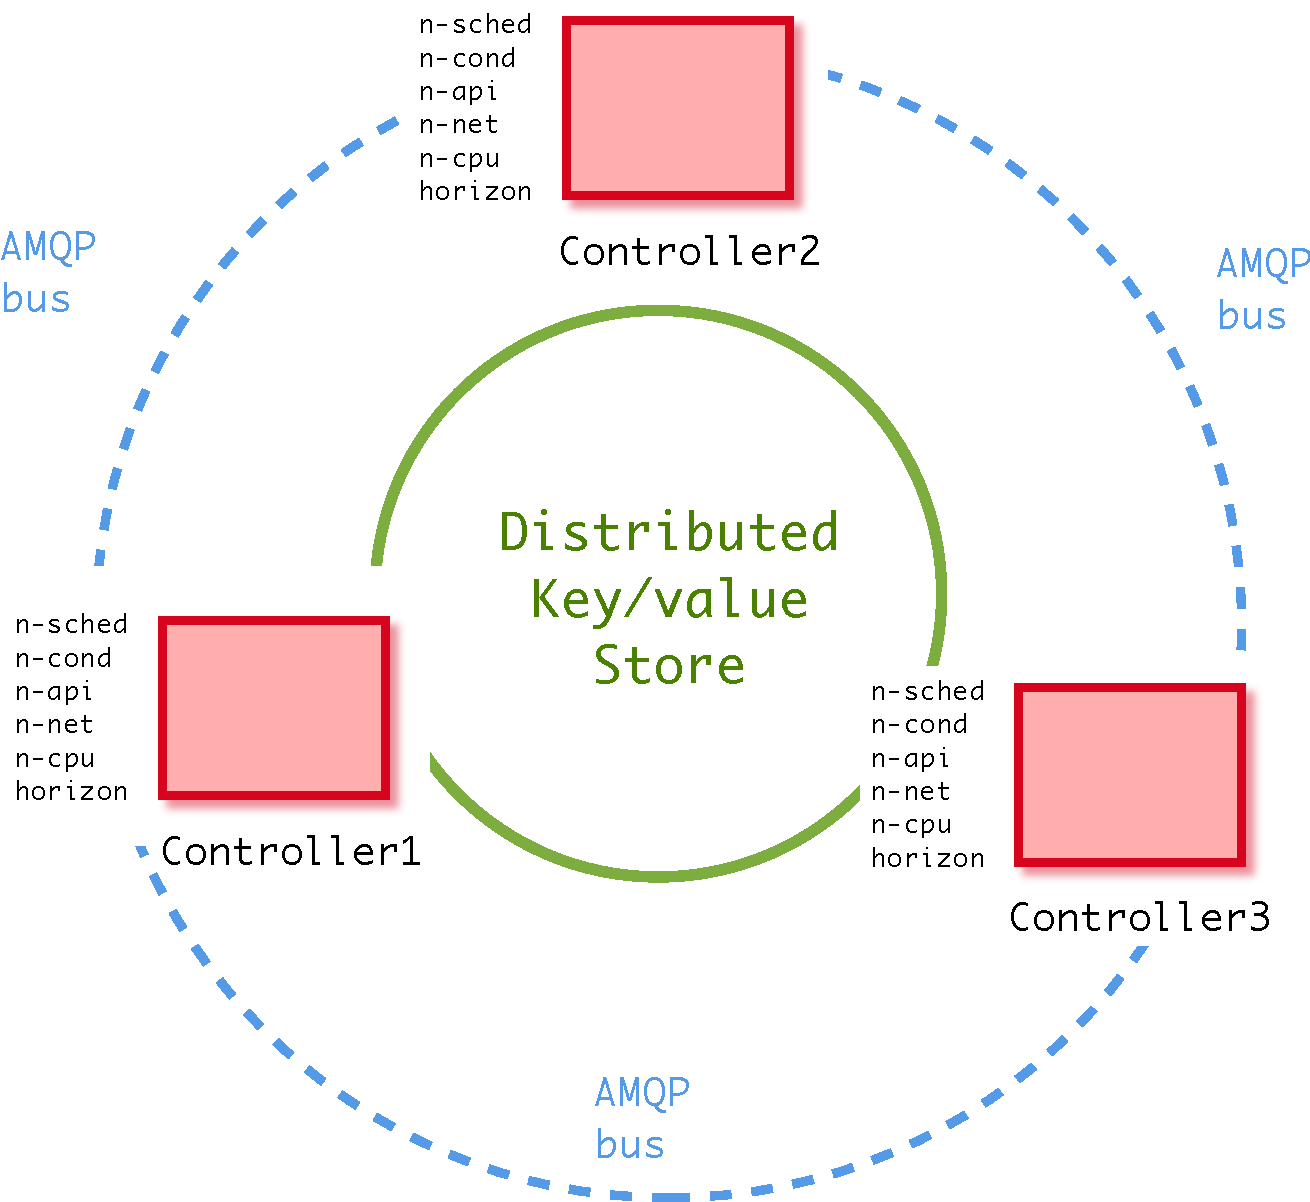
\includegraphics[width=6cm]{figures/OpenStack_distributed.pdf}
        \caption{Nova controllers are connected through a shared key/value backend
        and the AMQP bus.}
      \label{fig:newnova}
\vspace*{-.3cm}
\end{figure}

The architecture used for the Nova service has been organised in a way which
ensures that each of its sub-services does not directly manipulate the database:
they have an indirect access through a service called ``nova-conductor" which in
turn works with an implementation of the \textbf{"nova.db.api"} programming
interface. Developers of Nova provide an implementation of this interface that
is using \textit{SQLAlchemy} to manipulate a relational database. We developed a
second implementation of this interface that replaces every call to the
\textit{SQLAlchemy} by a call to a custom RIAK driver. This enables to make
Nova's services working with RIAK by only changing the database driver: this
limits the level of intrusiveness in the original source code.
